\documentclass[output=paper,colorlinks,citecolor=brown,
% hidelinks,
% showindex
]{langscibook}

\author{Víctor Acedo-Matellán\affiliation{University of Oxford} and Josep Ausensi\affiliation{Universitat Pompeu Fabra} and  Josep M. Fontana\affiliation{Universitat Pompeu Fabra} and  Cristina Real-Puigdollers\affiliation{Universitat Pompeu Fabra}}
\title{Old Spanish resultatives as low depictives}

\abstract{In this paper, we propose an analysis of a construction found in Old Spanish corpora that can at first sight be identified with an adjectival resultative construction (cf. \textit{John shot him dead}), e.g., \textit{lo abatió a tierra muerto}, lit. ‘they knocked him down dead’. The alleged existence of adjectival resultative constructions in Old Romance varieties is puzzling, since they are absent in earlier varieties (Latin) or Modern Romance varieties. We provide evidence that these constructions are not true adjectival resultative constructions.  Our main claim is that these constructions are a type of low depictive attached to the resultative layer within the VP, adopting the framework of transitions developed in \citet{Acedo-Matellan2016}, and a modified version of the theory of depictives, as put forth in \citet{Pylkkanen2008}. In doing so, we offer an analysis of a type of construction that appears in old varieties of Spanish and disappears later on.  All in all, the distribution of the constructions studied here depends on a different set of conditions, crucially not related to the satellite/verb-framed parameter. In addition, this study contributes to the understanding of secondary predication from a diachronic perspective.}

\IfFileExists{../localcommands.tex}{%hack to check whether this is being compiled as part of a collection or standalone
   \usepackage{langsci-optional}
\usepackage{langsci-gb4e}
\usepackage{langsci-lgr}

\usepackage{listings}
\lstset{basicstyle=\ttfamily,tabsize=2,breaklines=true}

%added by author
% \usepackage{tipa}
\usepackage{multirow}
\graphicspath{{figures/}}
\usepackage{langsci-branding}

   
\newcommand{\sent}{\enumsentence}
\newcommand{\sents}{\eenumsentence}
\let\citeasnoun\citet

\renewcommand{\lsCoverTitleFont}[1]{\sffamily\addfontfeatures{Scale=MatchUppercase}\fontsize{44pt}{16mm}\selectfont #1}
  
   %% hyphenation points for line breaks
%% Normally, automatic hyphenation in LaTeX is very good
%% If a word is mis-hyphenated, add it to this file
%%
%% add information to TeX file before \begin{document} with:
%% %% hyphenation points for line breaks
%% Normally, automatic hyphenation in LaTeX is very good
%% If a word is mis-hyphenated, add it to this file
%%
%% add information to TeX file before \begin{document} with:
%% %% hyphenation points for line breaks
%% Normally, automatic hyphenation in LaTeX is very good
%% If a word is mis-hyphenated, add it to this file
%%
%% add information to TeX file before \begin{document} with:
%% \include{localhyphenation}
\hyphenation{
affri-ca-te
affri-ca-tes
an-no-tated
com-ple-ments
com-po-si-tio-na-li-ty
non-com-po-si-tio-na-li-ty
Gon-zá-lez
out-side
Ri-chárd
se-man-tics
STREU-SLE
Tie-de-mann
}
\hyphenation{
affri-ca-te
affri-ca-tes
an-no-tated
com-ple-ments
com-po-si-tio-na-li-ty
non-com-po-si-tio-na-li-ty
Gon-zá-lez
out-side
Ri-chárd
se-man-tics
STREU-SLE
Tie-de-mann
}
\hyphenation{
affri-ca-te
affri-ca-tes
an-no-tated
com-ple-ments
com-po-si-tio-na-li-ty
non-com-po-si-tio-na-li-ty
Gon-zá-lez
out-side
Ri-chárd
se-man-tics
STREU-SLE
Tie-de-mann
}
    \bibliography{localbibliography}
    \togglepaper[23]
}{}

\begin{document}
\maketitle

\section{Introduction}\label{sec:acedomatellan:1}
We analyze a particular type of construction found in Old Spanish (OSp) that bears a striking resemblance to the type of adjectival resultative constructions typically found in English (i.e., \textit{John shot him dead}). These data, illustrated in \ref{ex:acedomatellan:first}, are especially interesting and empirically relevant for current debates since, as is well-known, contemporary Romance languages are pure verb-framed languages, thus disallowing this type of adjectival resultatives.\footnote{The data used in this study come from several on-line historical corpora: \citet{Sanchez-Marcoetal2010} (hereafter, SM), \textit{Corpus del Español} (\citealt{Davies2002}) (hereafter, CES) and \textit{Corpus Diacrónico del Español} \citep{Corde} (hereafter, CORDE). All the source texts are from the 12th, 13th, 14th or 15th centuries. Initially, searches were restricted to cognates of the Old French verbs and adjectives discussed in \citet{troberg2014predicat} and were later extended to similar verbs/adjectives native to Ibero-Romance such as \textit{derribar} or \textit{derrocar} ‘knock down’. The dataset can be downloaded at: zenodo.org (include here doi). }

\ea\label{ex:acedomatellan:first}
  \ea
    \gll Et lo firio	de	vna	lança	por el 	uientre 	en	tal manera	lo derroco muerto del cauallo.\\ 
			and	\textsc{acc}.\textsc{m}.\textsc{3sg}	hit.\textsc{pfv}.\textsc{3sg}		of	a 		lance	on 	the 	belly	in	such	way \textsc{acc}.\textsc{m}.\textsc{3sg}	remove{pfv}.\textsc{3sg}	die.\textsc{ptcp}.\textsc{m}.\textsc{sg}		of.the	horse\\
    \glt Lit. `And the blow of his lance on his belly was such that he	knocked 			him dead off the horse.’ (Anonymous, \textit{Historia Troyana}, 1370; SM)
  \ex
    \gll Non 	la despoje desnuda e la dexe como  el dia 	en 	que    nasçio.	\\
			No		\textsc{acc}.\textsc{f}.\textsc{3sg}			strip.\textsc{sbjv}.\textsc{prs}.\textsc{3sg}			undress.\textsc{ptcp}.\textsc{f}.\textsc{sg}	and 	\textsc{acc}.\textsc{f}.\textsc{3sg}  	leave.\textsc{sbjv}.\textsc{3sg} like			the		day	in 		that 		born.\textsc{pfv}.\textsc{3sg}\\
    \glt `May he not strip her naked and leave her like the day she was born.’ (Anonymous, \textit{Biblia romanceada}, 1350; SM)
  \z 
\z 

Building on \citeauthor{Acedo-Matellan2010}'s (\citeyear{Acedo-Matellan2010, Acedo-Matellan2016}) reappraisal of \citeauthor{Talmy1991}'s (\citeyear{Talmy1991,Talmy2000}) typological classification, we distinguish two main classes of languages depending on how they express the change of location/state subevent that we label as Path (following \citealt{Acedo-Matellan2010,Acedo-Matellan2016}; \citealt{Acedo-MatellanandMateu2013}): satellite-framed languages and verb-framed languages. In satellite-framed languages, Path can receive exponence through a non-verbal element \ref{ex:acedomatellan:sat}, while in verb-framed ones, Path is obligatorily expressed through the verb \ref{ex:acedomatellan:verb}.
\footnote{A reviewer notes that this claim is stronger than what \citeauthor{Talmy2000} proposed in his typology \citep{Talmy2000}, in which lexicalization patterns were conceived as tendencies. Even though we know that this is the case in classical \citeauthor{Talmy2000}’s typology,  we follow \citeauthor{Acedo-Matellan2016}'s (\citeyear{Acedo-Matellan2016}) reappraisal, where he notes that there is an asymmetry between satellite-framed and verb-framed languages such that the former allow both satellite-framed and verb-framed structures (e.g., verbs that encode path in English like \textit{exit}, \textit{enter}), while the latter only allow verb-framed structures. The reviewer also notes that there are some alleged counterexamples to our claim such as Sp. \textit{Volar al nido }‘he/she flew to the nest’, in which a manner of motion verb apparently licenses a directional PP. However, we think that these cases do not involve a manner verb combined with a directional satellite. In fact, the examples that we find in Spanish (and other Romance languages) always involve a verb that can be classified in a group of manner verbs that also encode ``forward motion’’ like jump, run or fly (\citealt{Nichols2008},  suggesting that the path component is still encoded in the verb, not in the preposition.  %Although some authors (e.g., \citeauthor{fabregas2007exhaustive} \citeyear{fabregas2007exhaustive}; see also \citeauthor{Beaversetal2010} \citeyear{Beaversetal2010} for more discussion) have claimed that expressions like Sp.\textit{ corrió a la farmacia} 
%`he ran to the pharmacy’ or Sp. \textit{voló al nido} 
%`it flew to the nest’ are examples of a manner verb licensing a directional preposition, it can be shown that neither the verbs nor the prepositions appearing in these constructions are pure manner-of-motion verbs or path prepositions (see \citeauthor{Real-Puigdollers2010} \citeyear{Real-Puigdollers2010}, \citeyear{RealPuigdollers2013}, for details).  
}

\ea
\settowidth\jamwidth{(Spanish)}
  \ea\label{ex:acedomatellan:sat}
  The boat floated into the cave. \jambox{(English)}
  \ex\label{ex:acedomatellan:verb}
    \gll La 	botella 	entró							en		la 		cueva 		flotando.	\\
			The	bottle			enter.\textsc{pfv}.\textsc{3sg}		in		the	cave			floating\\\jambox{(Spanish)}
    \glt `The bottle got into the cave floating.’ 
  \z 
\z 

It is important to note in the context of this discussion that neither strong adjectival resultatives nor so-called weak adjectival resultatives (\citealt{Washio1997}) (cf. \textit{The joggers ran the pavement thin} and \textit{John froze the soup solid}, respectively) are found in weak satellite-framed languages with adjectival agreement. Latin, the immediate ancestor of Old Romance languages, was no exception (\citealt{Acedo-Matellan2010, Acedo-Matellan2016}). Adjectival resultatives are, of course, also notably absent in pure verb framed languages such as Spanish or the rest of contemporary Romance varieties (cf. Spanish: *\textit{Juan fregó la mesa brillante} 
`Juan wiped the table shiny’ (\textsuperscript{OK} with reading ``Juan wiped the shiny table'')), with the exception of the specific type of construction which will be briefly discussed in \sectref{sec:acedomatellan:3} (e.g., \textit{fregar la mesa bien fregada} lit. `wipe the table well wiped’; \citealt{Armstrong2012}; \citealt{EspinalandMateu2018}). The alleged existence of adjectival resultative constructions in Old Romance is, thus, rather puzzling since, if these varieties had true adjectival resultatives, they would be displaying a type of construction which is one of the hallmarks of strong satellite-framed languages (e.g., English). Assuming that Romance languages can be placed at an intermediate point of a gradual typological change from a weak satellite-framed type of language to a verb-framed type, with mixed stages in between, the manifestation of these phenomena is rather unexpected, to say the least. 

The main claim of this paper is to argue that the types of constructions illustrated by the examples in \ref{ex:acedomatellan:first} were not true resultative constructions in the relevant sense but rather instances of a type of depictive secondary predication which was available in Old Romance and subsequently disappeared in the transition to contemporary Romance languages. We adopt a modified version of the Complex Predicate analysis of depictives put forth in \citet{Pylkkanen2008} and propose that these idiosyncratic depictive predicates are introduced by a specific kind of low applicative head, Dep\textsubscript{s}, which introduces a state and temporally links it with the result state entailed by the main verbal predicate. 

The structure of the paper is as follows. In \sectref{sec:acedomatellan:2}, we provide an overview of the resultative-like constructions found in OSp and argue that they are not true adjectival resultatives of the type found in satellite-framed languages. In \sectref{sec:acedomatellan:3}, we compare these constructions to similar constructions in Old French as well as to \textit{cognate} \textit{resultatives}, i.e., a different type of construction found both in old and contemporary Romance languages. In \sectref{sec:acedomatellan:4}, we develop a neoconstructioninst analysis for this type of constructions which treats them as low depictives rather than as true resultatives. In \sectref{sec:acedomatellan:5}, we briefly speculate about the diachronic path that led to the appearance and disappearance of this type of depictives in Spanish. Last, \sectref{sec:acedomatellan:6} concludes the paper.

\section{Adjectival resultatives in Old Spanish}\label{sec:acedomatellan:2}

The first piece of evidence that the constructions under discussion are not true adjectival resultatives comes from the fact the adjective is an adjunct. This is illustrated by examples like the following ones, where we can see that the adjective \textit{dead} can appear with other modifiers expressing other results, e.g., \textit{en tierra} ‘on the ground’ or it may not appear at all, with no apparent changes on the event-structure interpretation of the verb (cf. \textit{derribo} `knocked down' in \ref{ex:acedomatellan:galaz}).

\ea
  \ea
    \gll Derrocolo muerto en tierra\\
knock-down.\textsc{pfv}.\textsc{3sg}=\textsc{acc}.\textsc{m}.\textsc{3sg} die.\textsc{ptcp}.\textsc{m}.\textsc{sg} on ground\\
    \glt Lit. `He knocked him down dead on the ground.' (Anonymous, \textit{Gestas del rey don Jayme de Aragon}, 1396; CORDE)
  \ex
    \gll \&  derribo lo del cauallo  muerto en tierra. \\
and knock.down.\textsc{pfv}.\textsc{3sg} \textsc{acc.m.3sg}	of.the horse die.\textsc{ptcp}.\textsc{m}.\textsc{sg} on ground		\\
    \glt Lit. `He knocked him down dead on the ground.’ (Anonymous, \textit{Gran conquista de Ultramar}, 1290; SM)
  \ex\label{ex:acedomatellan:galaz}
    \gll Como Galaz derribo a Dalides de la lança. \\
    how Galaz knock.down.\textsc{pfv}.\textsc{3sg} \textsc{dom} Dalides of the spear\\
    \glt `How Galaz knocked Dalides down with the spear.' (Anonymous, \textit{La demanda del Sancto Grial}, c. 1470; CORDE)
  \z 
\z 

%\bg. la derribó muerta a los pies de Flosarán\\
%ACC.3SG.F knock-down.3SG.PFV dead.PTCP.3SG.F to the.3PL.M foot.PL.M of Flosarán\\
%Lit. `She was knocked down dead to Flosarán's feet.' (16th c., CES) %SEGLE 16%

Second, these constructions also diverge from weak adjectival resultatives (\citealt{Washio1997}) in permitting adjectives that introduce a result state distinct from the one encoded by the verb.\footnote{\citet{Washio1997} originally proposed to differentiate between weak and strong resultatives. In contrast with strong resultatives, where the verb does not encode any result state, in weak resultative constructions the main verb encodes a result state and the result phrase simply provides further specification about it (e.g., \textit{freeze something solid}). It is important to note in the context of this discussion that modern Spanish does not exhibit the type of constructions that are typically considered weak resultatives. Thus, the Spanish equivalents of \textit{I froze the ice cream solid/hard}, \textit{I wiped the table dry} or \textit{He sharpened the pencil pointy} are out.} Thus, whereas \textit{derribar} or \textit{derrocar}
`knock-down’ encode a change along a location scale (i.e., a change of location), \textit{muerto} `dead’ in the previous example or \textit{tollido} `crippled' in the example below denote changes along property scales (\citealt{Beavers2011}), namely a change of state.

%\ag. los derriba mortalmente feridos\\ AQUEST EXEMPLE EL REPETIM A SOTA
%ACC.3PL.M knock-down.3SG.PRS deadly hurt.PTCP.3PL.M\\
%Lit. `He knocks them down deadly injured.' (13th c., CES)
\ea
  \gll Tollidos los derribó de los cavallos en el campo.\\
crippled.\textsc{ptcp}.\textsc{m}.\textsc{pl} \textsc{acc}.\textsc{m}.\textsc{3pl} knock-down.\textsc{pfv}.\textsc{3sg} of the horses in the field\\
  \glt Lit. `He knocked them down crippled off the horses in the field.' (Garci Rodríguez de Montalvo, \textit{Amadís de Gaula} [Books I and II], 1482--1492; CORDE)
\z 

%\bg. la derribo quasi muerta en el suelo.\\
%\textsc{acc.f.3sg} knocked.down almost dead.\textsc{f.sg} in the floor\\
%Lit. `He knocked her down almost dead on the ground.' (Juan de Flores, \textit{Grimalte y Gradisa}, c. 1495; CORDE)

Third,  the adjectives typically appearing in these constructions clearly display participial properties (see \citealt{Bosque1990}) and they can be found in the corpus as part of passive constructions.

\ea\label{ex:acedomatellan:ex1}
  \ea\label{ex:acedomatellan:asdrubal}
    \gll Fueron muertos por	 su 	hermano 	de Asdrubal.\\
be.\textsc{pfv}.\textsc{3pl}	die.\textsc{ptcp}.\textsc{m}.\textsc{pl}				by		his	 	brother 		of Asdrubal\\
    \glt Lit. `They were dead by his brother Asdrubal.' (Fernández de Heredia, \textit{Breviarium ab urbe condita}, 1377; SM) 
  \ex\label{ex:acedomatellan:passives2}
    \gll Fue desnuda y mal 	herida con escorpiones.\\
be.\textsc{pfv}.\textsc{3sg}		undress.\textsc{ptcp}.\textsc{f}.\textsc{sg} and 	badly hurt.\textsc{ptcp}.\textsc{f}.\textsc{sg}	with 	scorpions \\ 
    \glt Lit. `She was stripped naked and badly hurt with scorpions.' (Bernardo de Breidenbach; Martín Martínez de Ampiés tr., \textit{Peregrinatio in Terram Sanctam; Viaje siquier peregrinación de la tierra}, 1498; CES) 
  \z 
\z 

Participles such as those appearing in \ref{ex:acedomatellan:ex1}, i.e., \textit{muerto}, \textit{desnuda} or \textit{herida}, are a representative selection of the different participles that can also appear in the kind of construction we are examining. Evidence for their passive/eventive interpretation comes from the type and form of the auxiliaries involved and by the fact that they appear with agentive or causative modifiers, i.e., \textit{por su hermano de Asdrubal} `by Asdrubal’s brother’ in \ref{ex:acedomatellan:asdrubal} and \textit{con escorpiones} ‘with scorpions’ in \ref{ex:acedomatellan:passives2}. According to \citet{Anagnostopolou2003}, participles can be divided into two different basic types depending on their complexity: lexical participles and phrasal participles. The former do not allow manner adverbial modifiers and cannot appear in passives, while the latter can. Examples \ref{ex:acedomatellan:ex1} and \ref{ex:acedomatellan:ex2}, involving adverbial modification of the secondary predicate, show that these adjectives exhibit the properties of the latter type of participles.  

\ea\label{ex:acedomatellan:ex2}
  \ea
    \gll Mi primo, me ha vengado, que amos los cavalleros derribó malamente feridos.\\
my cousin \textsc{acc}.\textsc{1sg} has avenge.\textsc{ptcp} that both the knights knock-down.\textsc{pfv}.\textsc{3sg} badly injure.\textsc{ptcp}.\textsc{m}.\textsc{pl}\\
    \glt Lit. `My cousin has avenged me as he has knocked down both knights badly injured.'  (Anonymous, \textit{Tristán de Leonís}, 1501; CORDE)
  \ex
    \gll Los derriba mortalmente feridos.\\
\textsc{acc}.\textsc{m}.\textsc{3pl} knock-down.\textsc{prs}.\textsc{3sg} deadly hurt.\textsc{ptcp}.\textsc{m}.\textsc{3pl}\\
    \glt Lit. `He knocks them down deadly injured.' (Anonymous, \textit{Crónica Troyana} [BNM I733], 1490; CORDE)
  \z 
\z 

If \citet{Embick2004} is correct in assuming that participles denoting a resultative event cannot appear in true resultative secondary predication (cf. \textit{kick the door open} vs. \textit{*kick the door opened}), the data we are examining strongly suggest that we are dealing with a significantly different type of construction.\footnote{An anonymous reviewer questions that the OSp constructions at stake are so distinct from the weak resultatives in Japanese analyzed in \citet{Washio1997}. The OSp constructions differ substantially from both strong and weak resultatives (see also fn. 3). In strong resultatives, the main verb encodes an action that brings about the result state denoted by the result phrase. In the OSp constructions, the verb does not encode any action, but a change of location. More importantly, though, in weak resultatives, at least according to the ones in Japanese by \citeauthor{Washio1997}, the verb needs to encode a result state and the result phrase simply further specifies the state the verb encodes (e.g., \emph{paint something blue}). In the OSp constructions, the main verb generally describes a change along a path, whereas the result phrases denote a change of state. Thus, in this respect, they substantially differ from weak resultatives (as well as from strong resultatives) insofar as the meaning of the verb and the meaning of the result phrase is completely independent of each other (cf. \citealp{Washio1997}). }

Finally, another significant way in which the Old Romance construction we are examining clearly differs from canonical resultatives is that it clearly violates the well known general restriction against the simultaneous expression of more than one result state in a single clause (\citealt{Goldberg1991}; \citealt{Tenny1994}; \citealt{LevinAndRappaportHovav1995}; \citealt{Tortora1998}; \citealt{RappaportHovav2008}; \citealt{BeaversAndKoontz-Garboden2017}; \citealt{Ausensi2019a,Ausensi2021,Ausensi2020c}). This is illustrated by the contrast between the examples above and the acceptability of their English translations below. 

\ea
  \ea[\#] {The knight knocked him down dead to the ground.}
  \ex[\#] {The knight knocked them down crippled to the ground.}
  \ex[\#] {The queen knocked them down badly hurt to the ground.}
  \z 
\z 

In spite of the significant differences between the Old Romance constructions and canonical resultatives (weak or strong), there are admittedly also some rather striking similarities between them with respect to their interpretation. Even though the verbs in the OSp examples we have examined so far ostensibly encode a change of location, as the following example further illustrates, the contexts in which they are typically used strongly imply some sort of contact (e.g., a fight between two knights where one hits the other one and knocks him from the horse by hitting him with a lance) (see also \citet{trobergburnett} for Old French). Most significantly, the types of result phrases that are most frequent in these constructions are also restricted to a scale describing a change of state that is likely to result from the physical contact implied by the main verbs (e.g., \textit{muerto} `dead’, \textit{herido} `hurt’ or \textit{tullido} `crippled’).

\ea
  \gll  E tan gran ferida con su lança le dio, que lo derribó medio muerto.\\
and such big blow with his lance \textsc{dat}.\textsc{3sg} give.\textsc{pfv}.\textsc{3sg} that \textsc{acc}.\textsc{m}.\textsc{3sg} knock-down.\textsc{pfv}.\textsc{3sg} half die.\textsc{ptcp}.\textsc{m}.\textsc{sg}\\
  \glt Lit. `He hit him so hard with his lance that he knocked him down half dead.' (Pedro de Escavias, \textit{Repertorio de príncipes de España}, 1467--1475; CORDE)
\z  

Before proceeding any further, an important caveat is in order. While it is true that the contexts in which \textit{derribar} `knock down' is usually found imply contact, this does not mean that \textit{derribar} or  \textit{derrocar} (or most of the other verbs typically found in this type of construction) lexically entail contact. In other words, what is crucial here is that occurrence of a contact event is pragmatically inferred, rather than lexically entailed by the main predicate. In terms of lexical entailments, then, \textit{derribar} only denotes a caused change of location, even if in the context of medieval warfare the pragmatic inference of some contact being involved is strong. It is uncontroversial, thus, that despite the significant differences we have described with respect to their syntactic properties there are striking similarities in the semantic interpretation of the resultative-like Old Romance constructions and that of resultatives involving contact/impact predicates in satellite-framed languages like English (cf. \citealt{Boas2003}, \citealt{Beavers2011}). 


%In this sense, these OSp adjectival resultatives are semantically alike to those resultatives involving contact/impact predicates (\citealt{Boas2003}), present in satellite-framed languages like English (\citealt{Washio1997}; \citealt{Beavers2011}).

%\ex. \a. The knight beat the king to death.
%\b. John hit Tom unconscious. 
%\c. The blacksmith pounded the metal flat.

%Nevertheless, despite these similarities, which we believe to be superficial, OSp constructions show different syntactic properties, as expressed above, namely they feature a change of location verbal predicate (not a contact predicate), they allow for two distinct result phrases in the same clause, and crucially that the type of category involved in the result phrase is a participle, not an adjective.\footnote{An anonymous reviewer questions that the OSp constructions at stake are so distinct from weak resultatives in Japanese, as analyzed in \citet{Washio1997}. We note, however, that the OSp constructions differ substantially from both strong and weak resultatives for several reasons (see also fn. 2). In strong resultatives, the main verb encodes an action that brings about the result state denoted by the result phrase. In the OSp constructions, the verb does not encode any action, but a change of location. More importantly, though, in weak resultatives, at least according to the ones in Japanese by Washio, the verb  entails a result state and the result phrase simply further specifies the state the verb encodes (e.g., \textit{paint something blue}). In the constructions at stake, the verb generally describes a change along a path, i.e., a change of location, whereas the result phrases denote a change of state (e.g., \textit{muerto} `dead'). Thus, in this respect, they substantially differ from weak resultatives (as well as from strong resultatives) insofar as the meaning of the verb and the meaning of the result phrase is completely independent of each other (at least in Washio's terms). For these reasons, we focus specifically on the OSp constructions of the \textit{derribar muerto}-type insofar as they present a unique behavior with respect to both weak and strong resultatives.} Moreover, the fact that there is a coincidence between the non-literal meaning of these expressions in OSp and strong resultatives of the English type could be an extralinguistic factor playing a part in the paradigm.\footnote{ A possible explanation for that could be the introduction of a stylistic construction in medieval manuscripts taking as a model a Germanic language of the strong satellite-framed type. We leave this hypothesis, which we consider worth exploring, for future research. What is important for our purposes in this paper is that if this was indeed the case in OSp, the alleged resultative Romance construction would be built within a verb-framed system, yielding completely different syntactic properties. }

%Lastly, there are some outliers to the pattern depicted above in that we also find change of color resultatives (e.g., \textit{teñir} ‘dye’). %and predicates that do not seem to involve contact/impact, like \textit{vencer} ‘defeat’.
It is important to note at this point that there are also some apparent outliers to the patterns we are describing. Thus, in the texts of the same period we also find some instances of change of color resultatives (e.g., \textit{teñir} ‘dye’).

\ea
  \gll E preguntaron le por vn omne que tiñia su cabello negro \& por que lo fazia E dixo porque no le demanden sabiduria de los viejos.\\
and ask.\textsc{pfv}.\textsc{3pl} \textsc{dat}.\textsc{3sg} for a man that dye.\textsc{ipfv}.\textsc{3sg} his hair black and for that \textsc{acc}.\textsc{m}.\textsc{3sg} do.\textsc{ipfv}.\textsc{3sg} and say.\textsc{pfv}.\textsc{3sg} because no \textsc{dat}.\textsc{3sg} ask.\textsc{ipfv}.\textsc{3pl} wisdom of the old.\textsc{m}.\textsc{pl} \\
  \glt `And they asked him why that man dyed his hair black and he answered that this was because this man didn't want others to expect from him the wisdom old people are supposed to have.' (Anonymous, \textit{Bocados de oro}, 1250; SM)
\z 

%\bg. dieron batalla a los faliscos et los uencieron muertos.\\
%give.3PL.PFV battle to the.3PL.M faliscos and ACC.3PL.M defeat.3PL.PFV dead.PTCP.3PM.\\
%Lit. ``They fought the Faliscos and they defeated them dead." (14th c., SM)

%The case of \textit{vencer} predicates could be a case of spurious resultative since the adjectival result state cannot be understood as resulting from the event denoted by the main predicate, but rather as the manner with which the event of winning took place (cf. \textit{John cut the meat thin}).

\noindent We will leave out the analysis of the case of \textit{teñir} ‘dye’, since it has different properties (it features an adjective of color), it is not widely attested (only one case in the corpora consulted), and we can find examples of this type of resultative in Modern Romance, accepted by some speakers.\footnote{See \citet{Lawersetal2019} for a detailed analysis of color resultatives in French.}

\ea
  \gll ¡Pinta blanca la pared!\\
Paint white.\textsc{f}.\textsc{sg} the wall\\\jambox{(Modern Spanish)}
  \glt `Paint the wall white!'
\z 

 The most intriguing group of apparent outliers, however, is that made up of several examples involving the verbs \textit{batir} and \textit{ferir}, meaning ‘to beat’ or `to strike', (five and one instances, respectively, in the texts we examined) and a participle/adjective encoding what seems to be a resulting state.

\ea\label{ex:acedomatellan:batir+ADJ}
  \ea
    \gll E diol tan gran ferida, quel \textit{batio} \textit{muerto} del cauallo a tierra.\\
and give.\textsc{pfv}.\textsc{3sg}=\textsc{dat}.\textsc{3sg} so great blow that=\textsc{acc}.\textsc{m}.\textsc{3sg} knock.\textsc{pfv}.\textsc{3sg} dead.\textsc{ptcp.}\textsc{m}.\textsc{sg} from.the horse to ground\\
    \glt `And he hit him so hard that he knocked him off his horse and he wound up dead on the ground.’ (Anonymous, \textit{Historia troyana en prosa y verso}, c. 1270; CORDE)
  \ex
    \gll E diol Eneas tan gran lançada, que lo \textit{batio} \textit{muerto} del cauallo a tierra.\\
and give.\textsc{pfv}.\textsc{3sg}=\textsc{dat}.\textsc{3sg} Aeneas so great spear-blow that \textsc{acc}.\textsc{m}.\textsc{3sg} knock.\textsc{pfv}.\textsc{3sg} die.\textsc{ptcp}.\textsc{m}.\textsc{sg} from-the horse to ground\\
    \glt `And Aeneas struck him so hard with his lance that he knocked him off his horse and he wound up dead on the ground.’ (Anonymous, \textit{Historia troyana en prosa y verso}, c. 1270; CORDE)
  \ex
    \gll Et dieron al rey en el scudo dos pedraras et otra en el arçon et en las ancas de su cauallo et firieron muertos de los que eran con el.\\
And gave.\textsc{3pl} to-the king on the shield two stone-blows and another on the saddletree and on the haunches of his horse and struck dead of the who were with him \\
    \glt `And they hit the king's shield with two stones and with another one they hit the saddletree and the haunches of his horse. They also struck dead some of the people that were with him.’ (Juan Fernández de Heredia, \textit{Gran crónica de España, III} [BNM, ms. 10134], 1376; CORDE)
  \ex\label{ex:acedomatellan:nenjo}
    \gll Lo \textit{batio} nenjo a labieno \textit{muerto} en tierra.  \\
\textsc{acc}.\textsc{m}.\textsc{3sg} beat.\textsc{pfv}.\textsc{3sg} Nenius \textsc{dom} Labienus die.\textsc{ptcp}.\textsc{m}.\textsc{sg} in ground.\\
    \glt `Nenius knocked Labienus down dead on the ground.’ (Alfonso X, \textit{General Estoria} [Part V], 1284; CORDE)
  \z 
\z 

%\noindent Of all the examples of our corpus, these are the only ones for which there does not appear to be a straightforward argument not to consider them instances of strong adjectival resultative constructions of the English \textit{beat dead} type. They involve the activity verb, \textit{batir}, which does not license a resultative interpretation by itself, outside of its use as ‘whisk (eggs, a mixture)’ or ‘beat flat, mint’ (for metals and coins). On the contrary, the interpretation of \textit{batir} as is found in narrative texts is strictly that of an activity verb, as illustrated by the next examples.  

\noindent Of all the examples in our corpus, these are the only ones for which there does not appear to be a straightforward argument not to consider them instances of strong adjectival resultatives of the English \textit{shoot dead} type. As illustrated by the following examples, these are verbs that are etymologically related to unbounded predicates (i.e., activities and semelfactives) which, in most medieval texts, would be translation equivalents of English verbs such as 
`beat', `hit', `knock', or `strike'.

\ea
  \ea
    \gll \textit{Batién} los cavallos con los espolones.\\
beat.\textsc{ipfv}.\textsc{3pl} the horses with the spurs\\
    \glt `They spurred their horses forward.' (Anonymous, \textit{Mio Cid}, c. 1140; CORDE)
  \ex
    \gll Olio de olivas sacado d’ellas \textit{batiéndolas} con palo.\\
oil of olives taken.out	from=them beating=\textsc{acc}.\textsc{f}.\textsc{3pl} with stick\\
    \glt `Olive oil taken out of olives after beating them with a stick.'
(Alfonso X, \textit{General Estoria} [Part I], FOL. 204v, c. 1275; CORDE)
  \ex
    \gll firio el cauallo de las espuelas \& va contra tristan\\ 
struck the horse with the spurs and went against tristan \\
    \glt `He spurred his horse forward and rode against Tristan.' (Anonymous, \textit{Cuento de don Tristán de Leonís}, c. 1313; CORDE)
  \z 
\z 

\noindent We argue, however, that the examples in \ref{ex:acedomatellan:batir+ADJ} should not lead us to propose that they have been generated by a satellite-framed grammar, as that of English. The first observation to be made is that all of them but one \ref{ex:acedomatellan:nenjo} come from the same work, the \textit{Historia troyana en prosa y verso} (also known as \textit{Historia troyana polimétrica}, cf. \citeauthor{Larrea2012}'s \citeyear{Larrea2012} edition), an anonymous translation of the French XII c. epic poem \textit{Roman de Troie}, by Benoît de Sainte-More. Funnily enough, a thorough search of \textit{Le Roman de Troie} (in \citeauthor{Joly1871}'s \citeyear{Joly1871} edition) does not reveal any single example of a resultative construction (adjectival or not) with \textit{batir}’s French cognate \textit{battre}. Instead, all the adjectival resultative constructions found involve the prefixed counterpart \textit{abattre} ‘beat, knock down’, combined with either \textit{mort} ‘dead’ (in all cases except one) and \textit{plat} ‘flat, spread’ (one case) (see also \sectref{sec:acedomatellan:3}).

\ea
  \ea
    \gll Anceis auront M. chevaliers \textit{Abatuz} \textit{morz} de lor destriers.\\
before will.have.\textsc{3pl} thousand knights beaten.down.\textsc{m}.\textsc{pl} die.\textsc{ptcp}.\textsc{m}.\textsc{pl} from their horses\\
    \glt `Before that, they will have knocked down dead from their horses a thousand knights.’ (l. 5037–38)
  \ex
    \gll D’une grant lance que il tint Fiert Odenel si qu’il l’\textit{abat} Jambes levées, trestot \textit{plat}.\\
of=a great spear that he held.\textsc{3sg} hits Odenel so that=he him=beats.down legs lifted suddenly flat.\textsc{m}.\textsc{sg}\\
    \glt `With a great spear that he held, he hits Odenel, in such a way that he all of a sudden takes him down flat, his legs upright.’ (l. 9723–24)
  \z 
\z 

\noindent Quite on the contrary, \textit{Historia troyana en prosa y verso} (in \citealt{Larrea2012}) does not present a single instance of \textit{abatir}, the Spanish cognate of \textit{abattre}. We surmise, therefore, that in this work \textit{batir} functions as a synonym of \textit{abatir}. Since beyond these three examples, there is only one example left from a different work \ref{ex:acedomatellan:nenjo}, and since, as pointed out by \citeauthor{Corominas1984} (\citeyear{Corominas1984}: s. v. \textit{batir}), this verb is quite scarce in Spanish, as opposed to Occitan-Catalan Romance and Gallo-Romance, we claim that the four examples in  \ref{ex:acedomatellan:batir+ADJ} do not amount to compelling evidence for a strong satellite pattern of adjectival resultatives being active in OSp.

 
\section{Resultative constructions in Old French and Modern Romance}\label{sec:acedomatellan:3}

 A considerable amount of research has been devoted to the expression of resultativity in Old French. The earliest studies in this area examined the productive use of verbal prefixes to convert activity predicates into telic predicates (e.g., \citealt{buridant1995preverbes, buridant2000nouvelle}; \citealt{dufresne2001changement, dufresne2003preverbs}; \citealt{kopecka2009continuity}). Beyond the expression of resultativity through verbal prefixes, however, \citet{trobergburnett} and \citet{TrobergandBurnett2017} have also argued for a characterization of Medieval French as a chronolect showing unprefixed resultative constructions involving PPs/particles \ref{ex:acedomatellan:2} and adjectives \ref{ex:acedomatellan:3}.

%\ex.	Old French; \citep{dufresne2003preverbs}
%\ag.	pens-er; s’a-pens-er \\
%think-\textsc{inf};	\textsc{refl}=at-think-\textsc{inf}\\
%‘to think’; ‘to realize’
%\bg.	am-er;		en-am-er \\
%		love-\textsc{inf};  in-love-\textsc{inf}\\
%		‘to love’; ‘to fall in love’
%\bg.	piss-er;		con-piss-er \\
%		piss-\textsc{inf};	with-piss-\textsc{inf}\\
%‘to piss’; ‘to cover with piss’

\ea
  \ea\label{ex:acedomatellan:2}
    \gll Et puys après nous troterons en guerre.	\\
and then after we will.trot in war\\
    \glt ‘And then after we will trot into war.’ (De La Vigne, \textit{La Ressource de la Chrestienté}, 1494, 133; DMF, \textit{apud} \citeauthor{TrobergandBurnett2017} \citeyear{TrobergandBurnett2017}: 112)
  \ex\label{ex:acedomatellan:3}
    \gll que	mort	ne	l’acraventet \\
that	dead	not	him=crush\\
    \glt ‘that it didn’t crush him dead’ (Roland, c.1100, 285.3930; MCVF; \textit{apud} \citep[114]{TrobergandBurnett2017} 
  \z 
\z 

The fact that these structures are found in the Old French texts is significant, since Modern French does not feature any of these three types of resultative constructions (see for example \citealt{FongandPoulin1998})

%Importantly, Modern French does not feature any of the three types of resultative constructions illustrated above, as had otherwise been shown by \citet{FongandPoulin1998}, among other authors.

%\ex.	Modern French; \textit{apud} \citeauthor{TrobergandBurnett2017} (\citeyear{TrobergandBurnett2017}: 115)
%\ag.	*Ils	a-volèrent	en 	France.\\
%they	to-flew		in	France\\
%\bg.	*Seigneur	Gauvain	est allé hors de son logement.\\
%Sir		Gawain	 \textsc{aux}	gone	out	of	his	lodgings\\
%\bg.	*L’oiseau vole sur les branches.\\
%			the=bird flies on the branches\\
%\bg.	*battre le metal plat.\\
%			to.beat the metal flat\\


In light of these data, and taking into account the results of \citet{Acedo-Matellan2010} for Early and Classical Latin, \citet{trobergburnett} propose a punctuated model of diachronic variation from Latin to Modern French in three stages, each of which exhibits a different resultative system:

 

\begin{enumerate}
	\item The Latin stage with resultatives involving prefixes and, optionally, also a PP \citep{Talmy2000}.

	\item The Old Romance stage with prefixed and unprefixed resultatives admitting PPs or APs.

	\item The final stage in which secondary predication resultatives, either prepositional and adjectival, are absent.
\end{enumerate}\par

\noindent Concomitantly, \citet{trobergburnett} also propose the following distribution of resultatives in Latin, Old Romance and Modern Romance as summarized in \tabref{tab:acedomatellan:1:frequencies}.


\begin{table}
\caption{\citet{trobergburnett}}
\label{tab:acedomatellan:1:frequencies}
 \begin{tabular}{l llll}
  \lsptoprule
Resultatives & Latin & Old Romance & Modern Romance\\
  \midrule
  Strong  &   No  &    No  &    No      \\
  Weak  &   No &   Yes  &    No     \\
  Prepositional & Yes (prefixed) & Yes & No\\
  \lspbottomrule
 \end{tabular}
\end{table}


In what follows, we qualify \citeauthor{trobergburnett}'s characterization of the second stage, i.e., that of Old Romance, as well as the validity of the correlations presented in Table 1. First, as shown by \citet{Acedo-Matellaninprep}, in the majority of examples provided in \citet{trobergburnett} and \citet{TrobergandBurnett2017} to argue for a satellite-framed pattern, the verb can be shown to already encode directionality/resultativity. As the authors themselves notice (\citeyear{TrobergandBurnett2017}: fn. 20) with respect to unprefixed directed motion constructions with PPs \ref{ex:acedomatellan:2}:

\begin{quotation}
``This system should allow robust occurrences of goal-of-motion constructions with strictly manner of motion verbs as we see in English (i.e., \textit{wiggle}, \textit{spin}, etc.); however, we have only been able to identify goal-of-motion with manner verbs that themselves imply translative movement. A potential problem with this proposal, therefore, is that it is not constrained enough.''
\end{quotation}

\noindent In other words, the kind of verbs used in PP and particle directed motion constructions in Old French can be argued to fit \citeauthor{Nichols2008}'s (\citeyear{Nichols2008}) characterization as manner verbs encoding ``forward motion"  (see \citealt{Real-Puigdollers2010} for examples from different modern Romance languages; see also \citealt{Acedo-MatellanandMateu2015}). Turning now to the kind of adjectival resultative constructions that we find in Old French, it is important to notice that, as we observed in the case of OSp, the verbs appearing in these constructions seem to be interpreted as change of state predicates. As \citet{trobergburnett} point out, while prefixed \textit{abattre} `beat down’ readily appears with result state adjectives such as \textit{plat} `flat’ in 45 cases, its unprefixed, atelic counterpart \textit{battre} `beat’ is not attested at all in the same constructions (see the discussion on \textit{battre} and \textit{abattre} in \sectref{sec:acedomatellan:2}). This leads the authors to claim that Old French featured weak adjectival resultative constructions, rather than the strong adjectival resultative type we find in English (e.g., \textit{hammer the metal flat}).

On closer examination, then, the Old French data do not seem to offer strong support for the hypothesis that Old Romance could have involved a grammatical system that differed so radically from a typological point of view from the systems that emerged in the subsequent stages of the evolution of these languages. On the contrary, what these data strongly suggest is that, at that stage, directionality/resultativity was already encoded in the verb \textit{qua} word. This result would thus converge with our own findings for OSp.  

We also believe that the picture presented in Table 1 above is not completely accurate. For one thing, as illustrated by the following examples, Modern Romance does exhibit some form of weak resultatives. These types of (extremely) weak resultatives (see \citealt{Whelpton2006} and \citealt{Mateu2012}) known as \textit{cognate resultatives} can be found in most contemporary Romance varieties. 

\ea
\settowidth\jamwidth{(Spanish)}
  \ea\label{ex:acedomatellan:omplir}
    \gll Omplir l'ampolla ben plena.\\
fill the=bottle well full\\\jambox{(Catalan)}
    \glt `to fill the bottle well/really filled/full.’ \citep{EspinalandMateu2018}
  \ex\label{ex:acedomatellan:lavadita}
    \gll Lavó la camisa bien lavadita.\\
Washed the shirt well washed.\textsc{dim} \\\jambox{(Spanish)}
    \glt `She washed the shirt thoroughly.’ (\citealt{Demonte1991} \textit{apud} \citealt{Armstrong2012})
  \ex
    \gll Ho stirato la camicia piatta piatta.\\ 
have ironed the shirt flat flat.\\\jambox{(Italian)}
    \glt `I ironed the shirt [very flat].'  \citep{Napoli1992}
  \z 
\z 

\noindent In the following example from OSp, we can see an instance of this type of cognate resultative involving \textit{alçar} `lift' and the cognate adjective \textit{alto} `high'. Similar examples can also be found in Old French.

\ea\label{ex:acedomatellan:etancta}
  \gll E tancta era la undosa comoçión de aquella parte, que los \textit{alçava} tan \textit{altos} que parescían legar al çielo. \\
and so.great be.\textsc{ipfv}.\textsc{3sg} the waving commotion of that part that \textsc{acc}.\textsc{m}.\textsc{3pl} lift.\textsc{ipfv}.\textsc{3sg} so high.\textsc{m}.\textsc{pl} that seem.\textsc{ipfv}.\textsc{3pl} arrive.\textsc{inf} at.the sky\\
  \glt `And the waving movement on that spot was so great, that it lifted them so high that they seemed to reach the sky.' (Enrique de Villena, \textit{Traducción y glosas de la Eneida} [Books I-III], 1427--1428; CORDE)
\z 

The properties of this characteristic type of resultative construction can be summarized as follows:

%\noindent Rather, we add, the kind of verbs used in PP and particle directed motion constructions in Old French can be argued to fit \citeauthor{Nichols2008}'s (\citeyear{Nichols2008}) characterization as manner verbs encoding ``forward motion"  (see \citealt{Real-Puigdollers2010} for examples from different modern Romance languages; see also \citealt{Acedo-MatellanandMateu2015}). As regards the kind of adjectival resultative constructions that we find in Old French, the verbs appearing in these constructions seem to already be interpreted as change of state themselves. Thus, for instance, \citet{trobergburnett} point out that while prefixed \textit{abattre} `beat down’ readily appears with resultant state adjectives such as \textit{plat} `flat’ in 45 cases, its unprefixed, atelic counterpart \textit{battre} `beat’ is not attested at all in the same constructions (see the discussion on \textit{battre} and \textit{abattre} in the \textit{Roman de Troie} in \sectref{sec:acedomatellan:2}). This leads the authors to claim that Old French featured weak adjectival resultative constructions, in \citeauthor{Washio1997}'s (\citeyear{Washio1997}) terminology, rather than strong adjectival resultative constructions as we find in English (e.g., \textit{hammer the metal flat}).

%In conclusion, a close examination of Old French does not support, for Old Romance in general, the scenario with a completely new system different from Modern French: in both stages of the language, directionality/resultativity are encoded in the verb \textit{qua} word. This result converges with our findings for OSp.  Concomitantly, \citet{trobergburnett} provide the following distribution of resultatives in Latin, Old Romance and Modern Romance:

%\begin{table}
%\caption{\citet{trobergburnett}}
%\label{tab:acedomatellan:1:frequencies}
 %\begin{tabular}{l rrrr}
 % \lsptoprule
%Resultatives & Latin & Old Romance & Modern Romance\\
 % \midrule
 % Strong  &   No  &    No  &    No      \\
 % Weak  &   No &   Yes  &    No     \\
 % Prepositional & Yes (prefixed) & Yes & No\\
  %\lspbottomrule
 %\end{tabular}
%\end{table}

%\noindent We believe the picture presented in the table above is not completely accurate, since Modern Romance displays a type of (extremely) weak resultatives, although, crucially, with very different properties as the ones discussed in \sectref{sec:acedomatellan:1} and \sectref{sec:acedomatellan:2}.

%\ex. \label{ex:acedomatellan:omplir} \ag. Omplir l'ampolla ben plena.\\
%fill the=bottle well full\\
%`to fill the bottle well/really filled/full.’ \citep{EspinalandMateu2018} {\hfill \raisebox{1.9\baselineskip}[0pt][0pt]{(Catalan)}} 
%\bg. Lavó la camisa bien lavadita.\\
%Washed the shirt well washed.\textsc{dim} \\
%`She washed the shirt well washed’. \label{ex:acedomatellan:lavadita} (\citealt{Demonte1991} \textit{apud} \citealt{Armstrong2012}) {\hfill \raisebox{2.9\baselineskip}[0pt][0pt]{(Spanish)}}
%\bg. Ho stirato la camicia piatta piatta.\\ 
%have ironed the shirt flat flat.\\
%`I ironed the shirt [very flat].'  \citep{Napoli1992} {\hfill \raisebox{1.9\baselineskip}[0pt][0pt]{(Italian)}}

%The properties of these type of resultative constructions in Modern Romance, which we label \textit{cognate resultatives} (see also \citealt{Whelpton2006}, \citealt{Mateu2012}), can be summarized as follows:


\begin{enumerate}
	\item They require verb-adjective root identity (although this is not completely accurate for Catalan, cf. \citealt{EspinalandMateu2018} or Italian, cf. \citealt{Napoli1992}). The restriction lies basically in the nature of the scale introduced by the resultative predicate: it has to coincide with the one which is lexically entailed by the main predicate.

	\item They appear with either manner or change of state predicates (quantized and non-quantized scales (\citealt{Beavers2011})) and predicates of contact. See \citet{EspinalandMateu2018} for a detailed list in Catalan.

	\item They require that the secondary predicate presents the result state as different in degree or manner from the one that would be entailed by the mere verb. This involves either the use of a Spanish \textit{bien}  `well’ adverb, diminutive morphology on the secondary predicate, reduplication, or some of these strategies simultaneously (see \ref{ex:acedomatellan:lavadita}).
\end{enumerate}\par

\noindent From what we have said so far, then, it seems clear that these types of constructions exhibit syntactic properties that clearly set them apart from the type of construction we introduced in the previous sections (i.e., the \textit{derribar muerto} `knock down dead' type of construction found in the OSp and Old French texts).  


%\noindent Interestingly, we have found one example in OSp that looks like a cognate resultative, involving \textit{alçar} `lift' and the cognate adjective \textit{alto} `high'.

%\exg. E tancta era la undosa comoçión de aquella parte, que los \textit{alçava} tan \textit{altos} que parescían legar al çielo. \label{ex:acedomatellan:etancta}\\
%and so.great be.\textsc{ipfv}.\textsc{3sg} the waving commotion of that part that \textsc{acc}.\textsc{m}.\textsc{3pl} lift.\textsc{ipfv}.\textsc{3sg} so high.\textsc{m}.\textsc{pl} that seem.\textsc{ipfv}.\textsc{3pl} arrive.\textsc{inf} at.the sky\\
%`And the waving movement on that spot was so great, that it lifted them so high that they seemed to reach the sky.' (Enrique de Villena, \textit{Traducción y glosas de la Eneida} [Books I-III], 1427-1428; CORDE)

%\noindent However, it is evident that the kind of constructions found in OSp and Old French of the \textit{derribar muerto} `knock down dead' type are different from the cognate ones illustrated in examples \ref{ex:acedomatellan:omplir}, or that in \ref{ex:acedomatellan:etancta}, for that matter. In the next section we provide a formal analysis of the former type. In \sectref{sec:acedomatellan:5}, we adopt the analysis put forth in \citet{Armstrong2012} based on \citeauthor{Haugen2009}'s (\citeyear{Haugen2009}) account of cognate objects, and we point out the differences with respect to the adjectival OSp constructions discussed here.


\section{Building low depictives in Old Spanish}\label{sec:acedomatellan:4}

In this section, we justify and develop an analysis of OSp constructions of the \textit{derribar muerto}-type as low depictive constructions. This analysis integrates the treatment of depictives as complex predicates defended in \citet{Geuder2000} and \citet{Pylkkanen2008} with the specific approach to argument/event structure we outline in \sectref{sec:acedomatellan:4-1}. We show that the characteristic properties exhibited by the OSp constructions and described in \sectref{sec:acedomatellan:2} as well as those discussed in \sectref{sec:acedomatellan:3} for Old French can be adequately accounted for under this analysis.

\subsection{A neoconstructionist approach to argument/event-structure}\label{sec:acedomatellan:4-1}

Our approach to the structure of events is based on the syntactic, neoconstructionist theory of argument/event structure in \citet{Acedo-Matellan2016}, in turn heir to a tradition from \citet{HaleAndKeyser1993, HaleAndKeyser2002} and \citet{Mateu2002}. We assume that basic functional heads that build argument/event-structures are \textit{v}, denoting an eventuality, and \textit{p}, denoting a spatial relation. Little \textit{p} comes in two varieties: Place, encoding a location/state, and Path, encoding a change of location/state. Little \textit{p} is thus underspecified for the expression of state/location, following \citeauthor{Mateu2002}'s (\citeyear{Mateu2002}) novel reduction of the A(djectival) category to the P(repositional) category (also a tradition assuming the so-called localist hypothesis, see \citealt{Gruber1965}; \citealt{Jackendoff1983}). Of especial relevance for this study are constructions denoting a transition, whose skeleton is as follows (a VoiceP introducing the external argument has been omitted).


\ea The basic functional heads.\\
\begin{tikzpicture}
\Tree [.vP  \textit{v} [.PathP  \textit{Path}  [.PlaceP \textit{Place}  ]  ] ]  
\end{tikzpicture}
\z

\noindent Functional heads are combined with non-relational elements like NP/DP or bare roots.

\ea Functional heads combined with non-relational elements.\\
\begin{tikzpicture}
\Tree [.VoiceP \qroof{El rey}.DP [.Voice' \textit{Voice} [.vP \textit{v} [.PathP \textit{Path} [.PlaceP \qroof{el cavallero}.DP [.Place' \textit{Place} [.$\surd$\textsc{derrib}-  ] ] ] ] ] ] ] 
\end{tikzpicture}
\z

\noindent The DP \textit{el cavallero} is the specifier of PlaceP, which hosts the root $\surd$\textsc{derrib}- as complement. As such, it is interpreted as the holder of the state of being ``toppled down". Since PlaceP is complement to Path, which introduces a transition, the state is interpreted as the result of a change, i.e., a result state. \citet{Acedo-Matellan2016} analyzes strong resultative constructions of the English type via the adjunction of a root to the eventive head \textit{v}.

\ea\label{ex:acedomatellan:represented}
  The king beat the knight dead. \\

\begin{tikzpicture}
\Tree [.VoiceP \qroof{The king}.DP [.Voice' \textit{Voice} [.vP [.v \textit{v} [.$\surd$\textsc{beat} ] ] [.PathP \textit{Path} [.PlaceP \qroof{the knight}.DP [.Place' \textit{Place} [.$\surd$\textsc{dead} ] ] ] ] ] ] ]
\end{tikzpicture}
\z

\noindent The root adjoined to \textit{v} (cf. also \citealt{Embick2004}, \citealt{McIntyre2004}, \citealt{Harley2005}) specifies the manner of the event, the way in which the origination of death is carried out, which in this case is by beating. As we have seen in previous sections, the types of resultatives exhibited both by contemporary and medieval Romance varieties are crucially not of the strong type represented by the structure in \ref{ex:acedomatellan:represented}.  Among the different kinds of explanations offered to account for these kinds of typological differences, our analysis adopts the general view represented by proposals such as those found in \citet{Klipple1997, MateuandRigau2002, Acedo-Matellan2016}. According to this general view, verb-framed languages such as those in the Romance family differ from satellite-framed languages in that the result of the eventuality (denoted in the previous example by the expression \emph{dead}) has to be encoded in the verb, thereby precluding the use of a manner root associated to the main predicate head.

\subsection{Old Spanish resultatives as low depictives}\label{sec:acedomatellan:4-2}
\subsubsection{Standard depictives vs. low depictives}\label{sec:acedomatellan:4-2-1}

The basic properties of the OSp \textit{derribar muerto}-type construction discussed in previous sections can be summarized as follows: (a) reliance on change of location/state verbs as the main predicate in the construction, (b) lack of dependence between the scales introduced by the main verb and those introduced by the secondary predicate and (c) non-iterability. While there may be weak resultatives and cognate resultative constructions that exhibit property (a), crucially, not only do these two specific types of resultative constructions differ from one another in relevant ways but they are also in turn both significantly different from the Old Romance constructions we are examining here. For one thing, they are not assumed to exhibit property (b) as one of their basic properties. Property (b) appears to be, however, one of the core properties of the Old Romance resultative construction. As for property (c), as is well known, this is a property which is typically exhibited by all kinds of adjectival secondary predicates, both depictives and resultatives. 

Perhaps a bit paradoxically, the combination of all these three properties is what makes the particular type of construction we are investigating bear some rather striking resemblances not only to canonical resultatives but also to prototypical depictive constructions. We already saw how the Old Romance constructions differ from prototypical resultative constructions (both weak and strong). There are also some interesting ways, however, in which they can be distinguished from prototypical depictives. 

In the most well studied types of depictive constructions, such as the one illustrated in \ref{ex:acedomatellan:Miguelcongelo} below, the secondary predicate does not typically identify a state that holds of the entity associated with the argument in virtue of the event described by the main predicate (i.e., a result state) but rather a state that holds of that entity for the whole duration of the event or even previous to that event. 

\ea \label{ex:acedomatellan:Miguelcongelo}
  \gll Miguel congeló cruda la verdura.\\
Miguel freeze.\textsc{pfv}.\textsc{3sg} raw the vegetables\\
  \glt `Miguel froze the vegetables raw.' (interpretation: the greens were raw when the freezing event started)
\z 

In contrast, as we saw in the introductory sections of this paper, the secondary predicate that appears in the type of construction we are discussing does identify a result state that holds of the relevant entities and this state is interpreted (via pragmatic inference) to be a direct consequence of the event described by the main predicate.

\ea\label{ex:acedomatellan:hector}
  \gll Y derribó muerto Héctor al cruel Anpimaco.\\
and knock-down.\textsc{pfv}.\textsc{3sg}	die.\textsc{ptcp}.\textsc{m}.\textsc{3sg} Héctor \textsc{dom}=the cruel Anpimaco\\
  \glt Lit. `And Héctor knocked the cruel Anpimaco down dead.’ (Juan de Mena, \textit{Homero romanzado}, 1442; CORDE) 
\z 

The contexts were this or the other examples discussed above typically appear make it clear that the referent of the internal argument is dead (or hurt or crippled) in virtue of the event encoded by the main predicate (in this case \textit{derribó} `knock-down'). In other words, reading the text where the example above is found it becomes immediately apparent that Amphimachus is not dead when Hector initiates the event of toppling him down but rather that he dies as an (in)direct consequence of that event. What is also true, however, is that the secondary predicate \textit{muerto} ‘dead’ encodes a state holding simultaneously with that encoded by the verb \textit{derribó}. We will clarify this statement in the next section when we make the relevant facts more explicit but this is the crucial observation that we will capitalize on to develop our analysis of these constructions as a special type of depictive.


\subsubsection{The structure of Old Romance low depictives}\label{sec:acedomatellan:4-2-2}
\citet{Pylkkanen2008} argues against small clause analyses of depictive secondary predicates (\citealt{Williams1980}). Instead, she proposes a complex predicate account thereof, i.e., an account where a functional head combines with both the secondary predicate and the main predicate to yield the desired semantics: the entailment that a state overlaps with the event encoded by the main predicate. \citet{Pylkkanen2008} adopts \citeauthor{Geuder2000}'s (\citeyear{Geuder2000}) semantics for this functional head, Dep, which we define in \ref{ex:acedomatellan:Dep}. 


\ea\label{ex:acedomatellan:Dep}
  $\lambda$f\textsubscript{$<$ e,$<$ s, t$> >$}.$\lambda$x.$\lambda$e. ($\exists$s) f(s, x) \& e \textsubscript{\LARGE \textdegree} s 
\z

Dep takes three arguments: a predicate of states, an entity, and an event. It involves the existential binding of the state such that it holds of the entity, and the overlapping (encoded via the \textsubscript{\LARGE \textdegree} operator) of the event and the state. 

Dep combines with the secondary predicate (\textit{tired}, in this case) yielding, by Functional Application, a predicate that denotes a state temporally associated with the event described by the main verb. Afterwards, the constituent DepP combines with the main predicate (\textit{see}) via Predicate Modification. This is possible since they have the same type ($<$ e,$<$ s, t$> >$). The last step is the merger of the internal argument, which saturates the entity argument. The overlapping function ensures that the ``the state of being tired"  overlaps with the event of ``seeing". Importantly, \citeauthor{Pylkkanen2008} shows how some languages like Finnish have dedicated morphology for depictive adjectives (see the essive marking on the adjective in \ref{ex:acedomatellan:raakana}), providing empirical evidence for this complex predicate approach and for the existence of a Dep functional projection.

\ea Finnish; \citeauthor{Pylkkanen2008} (\citeyear{Pylkkanen2008}: 24):\\
  \ea
    \gll Sö-i-n 			raa’a-n 		tomaati-n.\\
eat-\textsc{pst}-\textsc{1sg} 	raw-\textsc{acc} 		tomato-\textsc{acc}\\
    \glt `I ate a raw tomato.’
  \ex \label{ex:acedomatellan:raakana}
    \gll Sö-i-n 			tomaati-n 			raaka-\textit{na}.\\
eat-\textsc{pst}-\textsc{1sg} tomato-\textsc{acc} raw-\textsc{ess}\\
    \glt `I ate a tomato raw.’
  \z 
\z 

The derivation of a depictive in English following \citeauthor{Pylkkanen2008} would be as follows.

\ea
  \ea $\llbracket$Sue saw Peter tired$\rrbracket$ = $\lambda$x.$\lambda$e. seeing (e) \& agent (e, Sue) \& theme (e, Peter) \& ($\exists$s) tired (s) \& in (Peter, s) \& e \textsubscript{\LARGE \textdegree} s.
  \ex Syntactic analysis\\
\begin{tikzpicture}
\Tree [ Sue [  Voice  [ Peter  [ see [.DepP tired Dep  ]  ]  ]  ]  ]
\end{tikzpicture}  
\z\z

\noindent In order to adapt \citeauthor{Pylkkanen2008}'s (\citeyear{Pylkkanen2008}) analysis to the type of resultative constructions encountered in Old Romance, we need to minimally tweak the semantics of Dep. We need a DepP that can combine with a state-denoting rather than an event-denoting projection, and, in particular, with the one that denotes the result state. This we carry out by substituting a variable over states (s) for the variable over events (e) and introducing subindices to distinguish the two states. Let us call this modified version of Dep, Dep\textsubscript{s}.

\ea
  $\lambda$f\textsubscript{$<$ s,$<$ s, t$> >$}.$\lambda$x.$\lambda$s\textsubscript{1}. ($\exists$s\textsubscript{2}) f(s\textsubscript{2}, x) \& s\textsubscript{1} \textsubscript{\LARGE \textdegree} s\textsubscript{2}
\z

In combination with the approach to event structure outlined in \sectref{sec:acedomatellan:4-1}, this allows us to model the result state as a projection of its own, able to combine with DepP. That projection will be a PlaceP, in our terms. We show this with the analysis of the example in \ref{ex:acedomatellan:hector}.

\ea y derribó muerto Héctor al cruel Anpimaco.

\resizebox{\linewidth}{!}{
\begin{tikzpicture}

\Tree [.VoiceP \qroof{Héctor}.DP [.Voice' \textit{Voice} [. vP v [.PathP \textit{Path} [.PlaceP \qroof{al cruel Anpimaco}.DP [.PlaceP [.PlaceP \textit{Place} [.$\surd$\textsc{\textsc{derrib}-} ] ] [.DepP Dep\textsubscript{s} [.PlaceP \textit{Place} [.$\surd$\textsc{\textsc{muert}-} ] ] ] ] ] ] ] ] ]  
\end{tikzpicture}}
\z

\noindent The secondary predicate \textit{muerto} `dead’, encoded by PlaceP, which comprises Place and the root $\surd$\textsc{\textsc{muert}-}, is the first argument taken by Dep\textsubscript{s}. The second is the result state of the eventuality, namely that entailed by \textit{derribó} and encoded as the PlaceP that has the root $\surd$\textsc{\textsc{derrib}-} as a complement. The specifier of PlaceP is merged thereafter, satisfying the final argument of Dep\textsubscript{s}. The semantics up to now involves a state (encoded in [\textsubscript{PlaceP} Place $\surd$\textsc{derrib}-]) holding of the entity Amphimachus (\textit{al cruel Anpimaco}) and overlapping in time with another state, (encoded in [\textsubscript{PlaceP} Place $\surd$\textsc{\textsc{muert}-}]). Merger of Path on top of PlaceP introduces a transition, and [\textsubscript{PlaceP} Place $\surd$\textsc{\textsc{derrib}-}] is automatically interpreted as a result state, and, crucially, so is [\textsubscript{PlaceP} Place $\surd$\textsc{\textsc{muert}-}], i.e., \textit{muerto}, by inference. Thus, resultative secondary predicates in Old Romance receive this interpretation indirectly, by being temporally associated, via the overlapping function, with the real result predicate. 

The analysis put forward here thus accounts for the specific properties exhibited by this type of construction. First, only transition verbs, i.e., those verbs encoding a result state, accept resultative predicates in Old Romance. This follows quite naturally from the semantic specification of Dep\textsubscript{s}: it requires a state to be combined with the whole phrase Dep\textsubscript{s}P. Second, the scales introduced by the transition verb (e.g., \textit{derribar}) and the resultative predicate (e.g., \textit{muerto}) need not be of the same type, since there is no derivative connection between the roots, even though the state encoded in the secondary predicate is expected to be pragmatically compatible with that encoded by the verb. Finally, we also predict a lack of iterability in low-depictive predicates. Indeed if another Dep\textsubscript{s}P were introduced above PlaceP, it would still require to saturate both an entity and a state argument positions, where there is only just one internal argument and one result state available per transition predicate. This prediction is borne out by the OSp data. In fact none of the examples of our corpus shows two adjectives (outside, of course, of coordination cf. \textit{derribaron muchos cavalleros muertos y llagados a tierra} `[They] knocked many down dead and sored to the ground’, which would be perhaps expected under an adjunction approach). The attentive reader should recall, however, that what the examples do show is the coexistence of the resultative adjective with a PP encoding a goal or source location for the transition event, as seen in the next example.

\ea\label{ex:acedomatellan:loecho}
  \gll Lo echo muerto a 	tierra. \\
\textsc{acc}.\textsc{m}.\textsc{3sg} throw.\textsc{pfv}.\textsc{3sg} die.\textsc{ptcp}.\textsc{m}.\textsc{3sg} 	to 	ground\\
  \glt `He threw him dead to the ground.’ (Anonymous, \textit{Plutarch I}, 1370; SM)
\z 

Does this PP jeopardize the prediction that only one secondary predicate is allowed in these constructions? We do not think so. It is important to emphasize that, while we do not find iteration of APs, we do find iteration of PPs, one interpreted as a source of motion and the other as a goal of motion. Quite crucially, there does not seem to be any  apparent fixed relative order and one type of PP may appear without the other.

\ea
  \ea
    \gll Lo derribó malferido de 	su 	caballo 	a 	tierra.\\
\textsc{acc}.\textsc{m}.\textsc{3sg} 	knock-down.\textsc{pfv}.\textsc{3sg} 		badly-hurt.\textsc{ptcp}.\textsc{m}.\textsc{sg} 	of 		his horse			to 	ground\\
    \glt Lit. `He knocked him down badly hurt from his horse to the ground.’ (Lope García de Salazar, \textit{Istoria de las bienandanzas e fortunas}, 1471--1476; CORDE)
  \ex
    \gll Derrocolo 	muerto en 	tierra 	del cauallo.\\
knock-down.\textsc{pfv}.\textsc{3sg} 	die.\textsc{ptcp}.\textsc{m}.\textsc{sg} 	to 		ground 	of-the 	horse\\
    \glt Lit. `He knocked him down dead to the ground from his horse.’ (Anonymous, \textit{Gestas del rey don Jayme de Aragon}, 1396; CORDE)
  \ex
    \gll Derribólo muerto 	a 	sus 	pies.\\
knock-down.\textsc{pfv}.\textsc{3sg}=\textsc{acc}.\textsc{m}.\textsc{3sg}	die.\textsc{ptcp}.\textsc{m}.\textsc{sg}	to	his 	feet\\
    \glt Lit. `He knocked him down dead to his feet.’ (Garci Rodríguez de Montalvo, \textit{Amadís de Gaula} [Books I and II], 1482--1492; CORDE)
  \z 
\z 

%\bg. lo 	derroco 	muerto	d 	el 		cauallo.\\ %CREC QUE AQUEST ES POT TREURE, NO APORTA RES QUE NO APORTI JA (36a)
%ACC.3SG.M 	knock-down.3SG.PFV 	dead.PTCP.3SG.M 	of 	the 	horse\\
%Lit. `He knocked him down dead from the horse.’ (14th c., CORDE)

These patterns thus suggest that the resulting location PPs are adjuncts merged above PlaceP. This is reflected in the analysis of \ref{ex:acedomatellan:loecho}, below.

\ea Lo echo muerto a tierra.\\

\begin{tikzpicture}[scale=.9]
\Tree [.VoiceP \textit{pro} [.Voice' \textit{Voice} [.vP v [.PathP \textit{Path} [.PlaceP [.PlaceP [.\qroof{lo}.Cl ] [.PlaceP [.PlaceP \textit{Place} [.$\surd$\textsc{ech}- ] ] [.DepP Dep\textsubscript{s} [.PlaceP \textit{Place} [.$\surd$\textsc{muert}- ] ] ] ] ]  [.\qroof{a tierra}.PlaceP ] ] ] ] ] ] 
\end{tikzpicture}
\z


\section{Diachronic change in resultative constructions in Old and Modern Spanish}\label{sec:acedomatellan:5}


In the previous section we have claimed that the OSp constructions examined in this paper are not true resultative constructions in the relevant sense but rather a different type of construction that we called \emph{low depictive}, i.e., one involving a depictive secondary predicate that targets the result state entailed by the verb, rather than the whole
event (thus distinguishing it from run-of-the-mill object-oriented
depictives). Our analysis adopts  \citeauthor{Pylkkanen2008}’s (\citeyear{Pylkkanen2008}) approach to depictive constructions qua complex predicates, involving the use of a dedicated functional head, Dep.  The analysis outlined  offers  some considerable advantages over previous analyses of these phenomena from a diachronic perspective. The most obvious one is that it does not require us to posit the existence of what would look essentially as a strong-satellite-framed grammatical system as the intermediate stage in a gradual typological shift widely assumed to have taken place from weak-satellite-framed Latin towards pure verb-framed Romance. Quite on the contrary, the data we have examined in this paper strongly suggest that the OSp constructions of the \emph{derribar muerto} `knock down dead' type cannot be analyzed as real instances of the constructions known as strong resultatives in English or other languages. We conclude, therefore, that these kinds of syntactic configurations cannot be taken as evidence to support the hypothesis that medieval Romance languages could have gone through a period of transition in which they were essentially strong satellite-framed languages before the strong verb-framed systems currently in place were established.\footnote{At the moment, we do not have a typological or parametric theory of the availability of Dep\textsubscript{s}, and hence we are in no position to predict which languages (English or any other) will feature low depictives. Unfortunately, it is true that this impinges on any principled account of the transition from OSp (featuring Dep\textsubscript{s}) to Classical/Modern Spanish (not featuring Dep\textsubscript{s}). Any such account must await future research.} 

As one of the anonymous reviewers rightly points out, just showing that these characteristic types of constructions can be analyzed as low depictives does not provide much of a diachronic account of the structure in question. We believe, however, that it can pave the way towards a more plausible explanation of these and similar phenomena. Assuming, for instance,  \citeauthor{Borer1984}'s (\citeyear{Borer1984}) conjecture on the nature of crosslinguistic variation, whereby variation resides exclusively in the properties of functional heads, our proposal would allow for the modelling of diachronic variation in the licensing of low depictive constructions in terms of changes in the nature or composition of the syntactic-semantic properties of Dep. 

Nevertheless, at this stage of the research, we cannot offer a full-fledged diachronic account of low depictives. The main limitation that we   currently have is the lack of a clear picture of the distribution of the construction  in the different chronolects. We can only speculate that they may have in fact been possible in Latin, albeit quite marginally. The kinds of data that we have in mind were already discussed in \citeauthor{Kühner1912} (\citeyear{Kühner1912}: 239–240), and are considered by \citeauthor{Pinkster1995} (\citeyear{Pinkster1995}: 197–198), who points out the scarcity of the pattern, and described and analyzed by \citeauthor{Acedo-Matellan2016} (\citeyear{Acedo-Matellan2016}: 170–171, 211). We include the following relevant examples from \citeauthor{Kühner1912} (\citeyear{Kühner1912}: 239–240), as laid out and translated by \citeauthor{Acedo-Matellan2016} (\citeyear{Acedo-Matellan2016}: 170):

\ea
  \ea \label{ex:acedomatellan:submersas}
    \gll \textit{Submersas} \textit{obrue} puppas.\\
sink.\textsc{ptcp.pst.acc.f.pl} overwhelm.\textsc{imp} ship.\textsc{acc.pl}\\
    \glt `Overwhelm the ships so that they sink.’ (Verg. A. 1, 69, \emph{apud} \citealt{Acedo-Matellan2016}: 170)
  \ex
    \gll \textit{Tectos}que per herbam \textit{dis-ponunt} enses et scuta \textit{latentia} \textit{condunt}.\\
cover.\textsc{ptcp.acc.m.pl}=and through grass.\textsc{acc} separate-put.3\textsc{pl} sword.\textsc{acc.pl} and shield.\textsc{acc.pl} be.hidden.\textsc{ptcp.prs.acc.n.pl} lay.\textsc{3pl}\\
    \glt `They arrange the swords in different places, hidden in the grass, and they lay the shields out of sight.’ 
(Verg. A. 3, 236, \emph{apud} \citealt{Acedo-Matellan2016}: 170)
  \z 
\z 

In these exemples the participles (\textit{submersas} `sunk', \textit{tectos} `covered', \emph{latentia} `hidden') apparently identify a state that is concomitant with the resulting state encoded by the verb (\textit{obrue} `overwhelm', \textit{disponunt} `lay out separately', \textit{condunt} `lay down'). That interpretation, the fact that the secondary predicates are participles, and the fact that the main verbs are verbs of change of location/state, could indeed lead us to claim that these are constructions akin to the OSp ones that we are scrutinizing in this paper.\footnote{\citeauthor{Acedo-Matellan2016} (\citeyear{Acedo-Matellan2016}: 170, 211) presents two analogous examples in which the alleged secondary predicate is an adjective. However, as this author points out, a reading of the adjective as a modifier rather than a predicate cannot be excluded.} Another possible analysis, however, is one in which the state denoted by the participle is prior to the event denoted by the verb. In fact, \citeauthor{Rushton1916}'s (\citeyear{Rushton1916}: 267) translation of \ref{ex:acedomatellan:submersas} seems to go along these lines:
``sink and overwhelm the ships", i.e., ``overwhelm the ships that have been sunk". Given the uncertainty of the interpretation of the participles, the rareness of the construction, and its limitation to poetry, for the time being we hesitate to draw any robust conclusions about the relation between these Latin constructions and the type that we find in OSp.

With respect to the presence of low depictives in Modern Spanish, we  conclude that they are not attested in contemporary varieties. The only constructions that resemble resultatives in this chronolect are the ones discussed in \sectref{sec:acedomatellan:3}, which we have called cognate resultatives, \textit{Secó la ropa bien seca} `They dried the clothes well dried.’, i.e., the variety showing root identity between the verb and the adjective. As discussed in \sectref{sec:acedomatellan:3}, cognate resultatives manifest a substantially different set of properties. Crucially, from the semantic point of view, in the cognate type,  both the verb and the cognate adjective make reference to the same scale, contrary to what we have described in the OSp constructions. For this reason, we conclude that the two kinds of  constructions are different and must be assigned two independent analyses.  Space restrictions prevent us from engaging in a detailed discussion about the proper analysis of cognate resultatives, but see  \citet{Armstrong2012}  and \citet{EspinalandMateu2018}.

%For the cognate resultative we will assume that  \citet{Armstrong2012} is right in proposing that the root identity characteristic of cognate resultatives follows directly from an l-syntactic analysis (\citealt{HaleAndKeyser1993,HaleAndKeyser2002}) whereby an abstract adjective incorporates into the verbal head, the initial and the final copies being both pronounced (\citeauthor{Armstrong2012} \citeyear{Armstrong2012}: 25).\footnote{ We refer the interested reader to \citet{EspinalandMateu2018} for an alternative analysis to the one proposed by \citeauthor{Armstrong2012}'s (\citeyear{Armstrong2012}).}

%\exg. Secaron la ropa bien seca.\\
%dry.\textsc{pfv}.\textsc{3pl}	the 		clothes 	really 	dry.\textsc{f}.\textsc{sg}\\
%`They dried the clothes well dried.’\\
							
%\begin{tikzpicture}
%\tikzset{every tree node/.style={align=center,anchor=north}}
%\Tree [.\textit{v}P   \qroof{\textit{pro}.\textsc{3p}}.DP   [.\textit{v}' 
% [.\textit{v}   [.V  A\\\textit{sec}      V    ]   \textit{v}     ]   [.VP  \qroof{la ropa}.DP   [.V'  [.V A\\\sout{\textit{sec}}   V  ]  [.AP  Adv\\\textit{bien} [.AP   A\\\textit{sec}     ]  ]    ]           ]  ]        ]
%\end{tikzpicture}			

All in all, cognate resultatives in Modern Spanish are not constructions involving what we have called a low depictive adjective. The lack of low depictives in modern varieties of Spanish could be explained  by positing a change in the availability of Dep\textsubscript{s},   at some point in the passage of OSp to Modern Spanish.  Thus,  while the former allowed two varieties of Dep, i.e., one that establishes a relation between a state and an event and another that establishes a relation between two states, the latter only features the variety relating states to events (i.e., \citeauthor{Geuder2000}’s \citeyear{Geuder2000} and \citeauthor{Pylkkanen2008}’s \citeyear{Pylkkanen2008} original proposal). However, at this stage, we do not know how the presence or absence of Dep\textsubscript{s} relates to some other property of the language. Consequently, we cannot offer for the moment an accurate account that traces and explains the emergence and obsolescence of the constructions at hand. Further work is certainly required to clarify these issues.



\section{Conclusion}\label{sec:acedomatellan:6}

Our study provides arguments against the analysis of OSp constructions of the \emph{derribar muerto} `knock down dead' type as adjectival resultatives. Instead, we have argued that these constructions involve a type of low secondary depictive predication.  In doing so, we solve the puzzle of having an intermediate stage in the evolution from Latin to Modern Romance, in which there is a completely different construction that is not present either in weak satellite-framed languages (Latin) or verb-framed languages (Romance). As a result, contra proponents of gradual change \citep{stolova2008satellite,kopecka2009continuity,iacobini2011diachronic}, or proponents of punctuated change à la \citet{trobergburnett} or \citet{troberg2014predicat} in three stages, we argue that OSp and Modern Spanish do not belong to two significantly different types with respect to the expression of resultativity. The fact that the constructions studied in this paper  are not resultatives and the lack of clear examples of other directional and resultative constructions in OSp make us conclude that it is quite plausible that OSp was already a verb-framed language 

%Last, as an anonymous reviewer points out, if the present analysis is on the right track, then it removes OSp low depictives from the discussion involving the typological change from satellite-framed Latin to verb-framed Romance, as some authors have proposed (\citealt{Troberg2019}). In this respect, it would provide evidence that Old Romance is not typologically different from Modern Romance, contra previous claims in the literature that hold that Old and Modern Romance constitute two distinct types of verb-framed languages (\citealt{Troberg2019}).

In conclusion, the distribution of the constructions discussed in this paper is dependent on a particular condition involving the availability in some languages of what we have called low depictives, which is crucially not related to the satellite/verb-framed parameter. We leave for further research the question of whether this analysis can capture other cases of alleged weak adjectival resultative constructions in other verb-framed languages \citep{Washio1997}. If the analysis outlined here is on the right track, it could open the way to a better understanding of the distribution of secondary predication (both depictive and resultative) across languages and diachronically.


\section*{Acknowledgements}
This paper has greatly benefited from the comments provided by two anonymous reviewers, and from the discussions held at several events where the research was presented: 29th Colloquium on Generative Grammar (CGG29), 49th Linguistic Symposium on Romance Languages (LSRL49), and different seminars at the Centre de Lingüística Teòrica (CLT), Universitat Autònoma de Barcelona. Any remaining shortcoming is our own responsibility.

The first author acknowledges funding from the project ``Redes de variación microparamétricas en las lenguas románicas" (FFI2017-87140-C4-1-P) (Ministerio de Economía y Empresa, Spain).

The remaining authors acknowledge support from the project Connecting Conceptual and Referential Models of Meaning 2 (CONNECT 2) (PI: Louise McNally) from the Ministerio de Economía y Competitividad (FFI2016-76045-P;\\ 
AEI/MINEICO/FEDER, UE) and from an ICREA Academia award to Louise McNally.

\printbibliography[heading=subbibliography,notkeyword=this]

\end{document}
